\chapter{Common Design and Implementation Strategy}\label{ch:design-implementation}


\section{Mechanism Model}\label{sec:mechanism-model}

After a thorough research and analysis of the available mechanisms implementations, it was identified the common design aspects that are shared among them.
These aspects, turned components, form the foundation of the future mechanisms implementations and are represented in the Mechanism Model, as shown in Figure~\ref{fig:mechanism-model}.

The Mechanism Model is composed of the following components:
\begin{itemize}
    \item \textbf{Configuration}: Represents a set of policies that, in conjuction, define the mechanism's behaviour (e.g., maximum number of retries, maximum wait duration, etc.);
    \item \textbf{Asynchronous Context}: Represents the mechanism's execution context, responsible for state management and event emission in an asynchronous environment;
    \item \textbf{State}: Represents the internal state of the mechanism;
    \item \textbf{Implementation}: Applies the configuration to the mechanism's execution context.
    Represents the core component of the mechanism;
    \item \textbf{Registry}: Acts as a centralized container for storing and managing available mechanism implementations and their configurations.
    The registry allows access to mechanism implementations throughout the application and enables the reuse of configurations to create new mechanisms;
    \item \textbf{Events}: Both the Asynchronous Context and Registry components are responsible for emitting events.
    The Asynchronous Context component emits events related to the mechanism's execution, such as internal state transition changes.
    The Registry component emits events related to \textit{CRUD} operations performed in the registry.
    These events can be used for various purposes, such as logging and monitoring;
    \item \textbf{Metrics}: The mechanism's implementation component is responsible for recording metrics related to the mechanism's execution (e.g., number of retries, number of recorded failures, etc.).
    These metrics can be used for monitoring and analysis purposes;
    \item \textbf{Decorator}: The decorator is an extension of the Implementation component.
    It is based on Resilience4J~\cite{resilience4j} decorators, and provides a convenient way to wrap code blocks with the mechanism's behaviour;
    \item \textbf{Ktor Plugin}: Responsible for the integration of the mechanism implementation with the Ktor pipeline.
    The Configuration component is also used to create a specific plugin configuration,
    which can be used to extend the mechanism's behaviour and provide additional features in an HTTP context.
\end{itemize}

\begin{figure}[!htb]
    \centering
    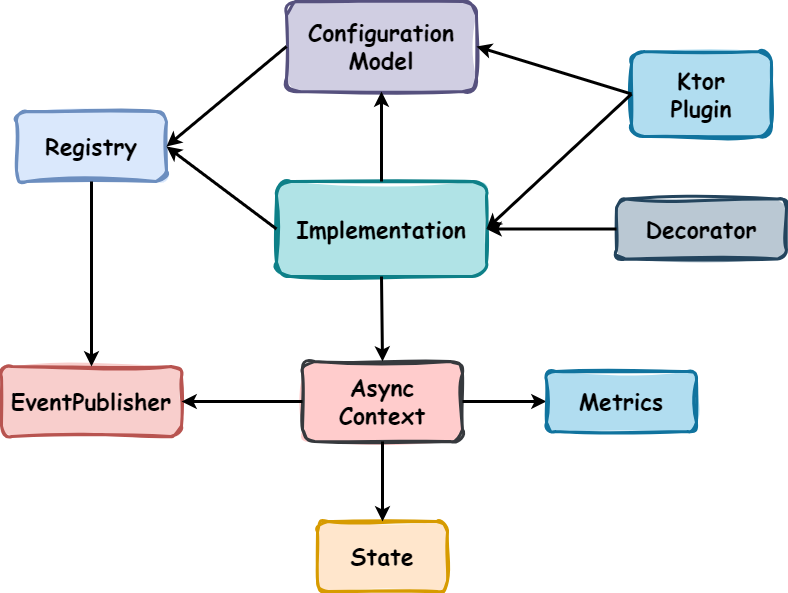
\includegraphics[width=0.8\textwidth]{../figures/03_mechanism-model}
    \caption{Mechanism Model}
    \label{fig:mechanism-model}
\end{figure}

\subsection{Configuration Design}\label{subsec:configuration-design}

Since the start of the project, the Configuration component has been designed to use the builder creational pattern~\cite{effective-java, design-patterns}, this way, separating the configuration definition (mutable) from the configuration usage (immutable).
However, this initial implementation had a limitation: it was not possible to override a configuration object (i.e., create a new configuration object based on an existing one, and only modify specific properties while keeping the rest of the properties unchanged).

To address this limitation, the Configuration component, particularly its builder,
was redesigned to always be constructed with a base configuration object.
This redesign enables incremental configuration, following a pattern where a configuration object is continually modified until the desired configuration is achieved.

The configuration process is as follows:

\begin{boldenumerate}
    \item Begin with a default or initial (base) configuration object;
    \item Pass this configuration to a configuration builder;
    \item The builder potentially modifies the base configuration;
    \item Generate a new configuration from the builder;
    \item If further modifications are needed, pass the new configuration back to the builder, which will use it as the base configuration;
    \item Repeat the process until the desired configuration is achieved.
\end{boldenumerate}

\subsection{Mechanism Execution Context}\label{subsec:mechanism-execution-context}

Independent of the execution environment, synchronous or asynchronous, the mechanism's execution context can only be one of the following:

\begin{itemize}
    \item \textbf{Per Mechanism}: A new execution context is created when the mechanism itself is instantiated (e.g., the Circuit Breaker mechanism has a single execution context for managing the circuit state, as multiple callers can interact with the mechanism at the same time);
    \item \textbf{Per Decoration}: When a decorator is applied to an operation, it creates a new execution context specific to that decoration, before invoking the underlying operation;
    \item \textbf{Per Method Invocation}: A new execution context is created each time the decorated method is invoked.
    This is the most granular form of execution context, providing isolation for each method call.
    If the underlying operation is thread-safe, then this form of execution context is also thread-safe, as only the calling thread executes the context (e.g., the Retry mechanism creates a new execution context for each underlying operation invocation).
\end{itemize}

\subsection{Asynchronous Context}\label{subsec:asynchronous-context}

Since the mechanisms are designed to be cross-platform, the execution context must be flexible and support asynchronous operations, particularly for JavaScript, one of the supported targets (see Section~\ref{sec:supported-targets}), which is single-threaded and requires asynchronous (non-blocking) operations.

In Kotlin, asynchronous operations are typically handled using Kotlin Coroutines~\cite{kotlin-coroutines},
which provide a way to write asynchronous code in a sequential manner,
leveraging the concept of suspending functions implemented using contination passing style (CPS)~\cite{continuation-passing-style}.

\subsubsection{Thread}\label{subsubsec:thread}

In computer science, a thread~\cite{java-thread} of execution is the smallest sequence of programmed instructions that can be managed independently by a scheduler, which is typically a part of the operating system.

In addition to being managed independently by an operating system's scheduler, threads are fundamental units of execution within a process.
They enable concurrent execution of tasks, allowing a program to perform multiple operations simultaneously.

\subsubsection{Kotlin Coroutines}\label{subsubsec:kotlin-coroutines}

A coroutine is an instance of a potentially suspendable computation,
which can be suspended and resumed at a later time (uses a state machine to manage its execution).
It is conceptually similar to a thread,
in the sense that it takes a block of code
to run that works concurrently with the rest of the code~\cite{kotlin-coroutines}.
However, a coroutine is not bound to any particular thread,
as it may suspend its execution in one thread and resume in another one.

A suspended coroutine does not block the underlying thread, freeing it to run other coroutines or perform other tasks.
In a thread, only one coroutine can run at a given time.

Another important feature of coroutines is that they enforce structured concurrency~\cite{kotlin-coroutines}.
Structured concurrency is a programming paradigm that enforces a hierarchical structure on concurrent code, ensuring that all concurrent tasks are properly managed and cleaned up, and any errors are propagated correctly and not lost.

\subsection{Event Publishing}\label{subsec:event-publishing}

Since the execution context is asynchronous, the events must be also published asynchronously.
To achieve this, the Kotlin Coroutines' asynchronous primitive Flow~\cite{kotlin-flow} was used to emit such events.

\subsubsection{Flow}\label{subsubsec:flow}

A Flow in Kotlin is a type of asynchronous data stream that can emit multiple values sequentially.
It is typically cold, meaning it starts emitting values only when collected,
ensuring that each collector receives the full sequence of values from the start.
In contrast, hot streams which emit values regardless of active collectors,
allowing multiple consumers
to observe ongoing data emissions~\cite{android-stateflow-sharedflow, kotlin-flow}.

Flows are distinct from Sequences~\cite{kotlin-sequences} in Kotlin.
While both can handle multiple values over time,
Flows are designed for asynchronous operations and do not block the calling thread when collecting values.
Sequences, however, are synchronous and computed on demand (lazy), blocking the calling thread during value computation.

\subsubsection{Implementation}\label{subsubsec:event-publishing-implementation}

In a mechanism, events are emitted using a hot Flow with no buffer, which means that, if there are no collectors (listeners) for the events, they are essentially lost (not recorded).
As such, a listener must be registered before the event is emitted, in order to receive it.

Each mechanism implementation has two ways to register listeners for events:

\begin{itemize}
    \item Receive all events emitted by the mechanism;
    \item Receive only a specific type of event emitted by the mechanism.
\end{itemize}

The implementation also provides a way to cancel all registered listeners by leveraging the coroutine's structured concurrency~\cite{kotlin-coroutines}, which is useful for cleaning up resources when the mechanism is no longer needed.
However, the cancellation of the registered listeners up to a given time does not affect later registrations.

\section{Decoration}\label{sec:decoration}

In mathematics,
function composition is an operation that takes two functions \textit{f} and \textit{g}, and produces a function \textit{h} = \textit{g} \textcircled{.} \textit{f} such that \textit{h}(\textit{x}) = \textit{g}(\textit{f}(\textit{x})).

In functional programming, a high-order function~\cite{higher-order-functions} is a function
that takes one or more functions as arguments and/or returns a function as its result.

A decorator is a structural design pattern
that attaches additional responsibilities to an object dynamically using aggregation/composition to provide a flexible alternative to subclassing for extending functionality~\cite{design-patterns}.

In the context of these mechanisms,
a decorator is a high-order function that wraps an operation
(e.g., method, function) with the behaviour of the mechanism.
The decorator needs to abide by the decoration principle,
which states that a decorator should not modify the operation's signature (i.e., name, parameters and return value), only alter its behaviour.
For callers of the operation, the decorator should be transparent (as if the operation was not decorated).

\subsection{Operation Types}\label{subsec:operation-types}

An operation represents a unit of work that can be decorated with the mechanism's behaviour (e.g., a function that makes an HTTP request).

In early development stages, the mechanisms were designed to support only one type of operation:
a function that takes no arguments and returns a value.
But this design was too restrictive, as it did not allow for operations that receive additional arguments.
To address this limitation, the operation types were redefined to support different scenarios:

\begin{itemize}
    \item \textbf{Supplier}: Accepts no arguments and produces a result.
    Based on Java's Supplier functional interface~\cite{java-supplier};
    \item \textbf{Function}: Accepts one argument and produces a result.
    Based on Java's Function functional interface~\cite{java-function};
    \item \textbf{BiFunction}: Accepts two arguments and produces a result.
    Based on Java's BiFunction functional interface~\cite{java-bifunction}.
\end{itemize}

Since the operations were going to be used in potential asynchronous contexts,
the operation types were redefined to be suspendable (i.e., representing potentially suspendable operations).

\subsection{Operation Context}\label{subsec:operation-context}

In later stages of development, it was considered to give the aforementioned operation types context-awareness,
meaning that the operations would have access to the mechanism's execution context in an immutable state
(i.e., for read-only purposes).

As a result, and to maintain backwards compatibility with the existing operation types (which allowed for method references~\cite{java-method-references} to be decorated), a new family of operation types was created with a \texttt{Ctx} prefix (e.g., \texttt{CtxSupplier}).
These new operation types receive the mechanism's execution context as an additional argument.


\section{Ktor Integration}\label{sec:ktor-integration}

Integration with Ktor presented an opportunity to apply the mechanisms in a real-world scenario
and validate their design and implementation.
But before integrating the mechanisms with Ktor, it is necessary to understand Ktor's architecture and how to extend its functionality using plugins.

\subsection{Plugin}\label{subsec:plugin}

In Ktor, a plugin is a reusable component that can be installed in an application to extend its functionality.
They represent a way to encapsulate common functionality (e.g., logging, authentication, serialization, etc.) and make it reusable across different applications.
Plugins are installed in the application's pipeline, where they can intercept and modify the request and response processing flow, as the Figure~\ref{fig:ktor-server-architecture} demonstrates for the server side.

\begin{figure}[!htb]
    \centering
    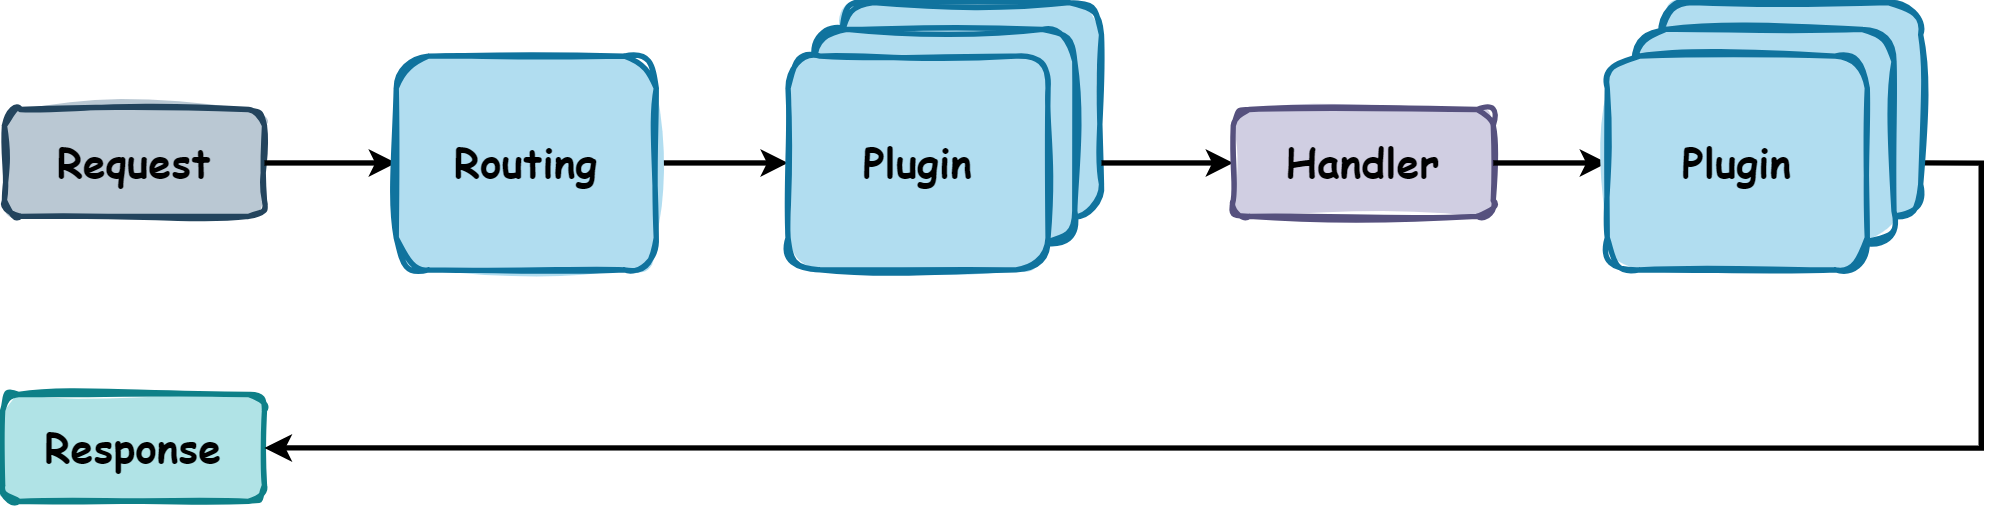
\includegraphics[width=0.8\textwidth]{../figures/03_ktor-server-architecture}
    \caption{Ktor Server Architecture}
    \label{fig:ktor-server-architecture}
\end{figure}

On the server side, as a request comes in, it goes through a series of steps~\cite{ktor-server-plugins}:

\begin{boldenumerate}
    \item It is routed to the correct handler via the routing mechanism (which is also a plugin);
    \item Before being handed off to the handler, it goes through one or more Plugins;
    \item The handler (application logic) handles the request;
    \item Before the response is sent to the client, it goes through one or more Plugins
\end{boldenumerate}

\subsection{Pipeline}\label{subsec:pipeline}

A Pipeline, represented in Figure~\ref{fig:ktor-pipeline}, is a collection of zero or more interceptors, grouped in one or more ordered phases.
Each interceptor can perform custom logic before and after processing a request.

\begin{figure}[!htb]
    \centering
    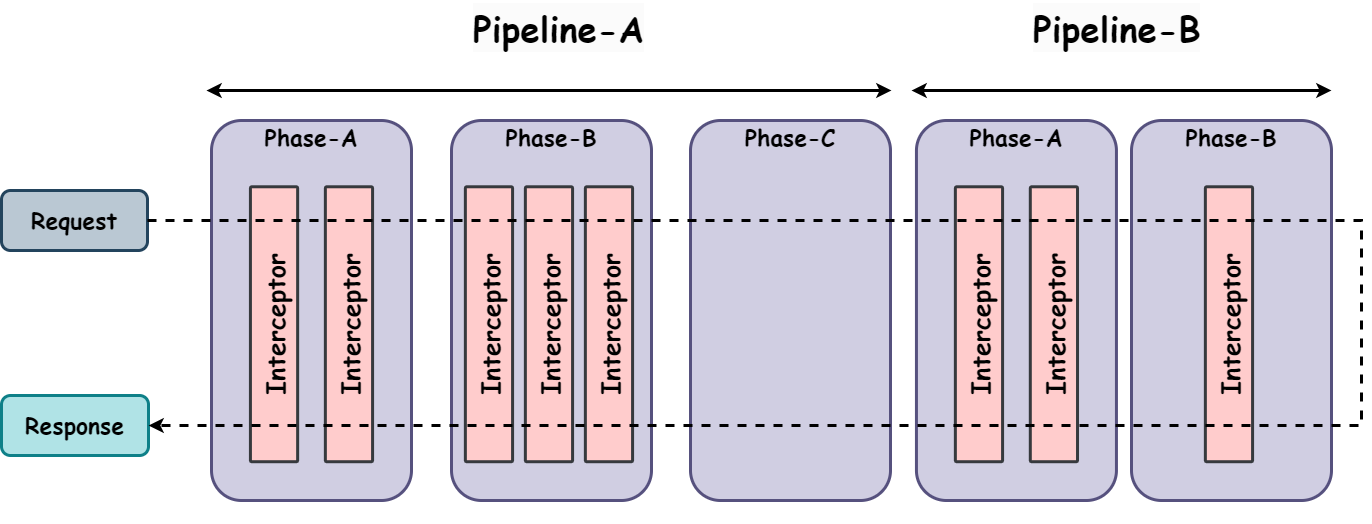
\includegraphics[width=0.8\textwidth]{../figures/03_ktor-pipeline}
    \caption{Ktor Pipeline Example}
    \label{fig:ktor-pipeline}
\end{figure}

A plugin is also an interceptor, but an interceptor is not a plugin.
An interceptor is a function block that can be added to intercept a specific pipeline phase and perform custom logic;
a plugin is a collection of zero or more interceptors mixed with external configuration and other logic
(e.g., add more pipeline phases) in a single reusable component.

Both client and server sides have pipelines, but they differ in number, phases, and purpose.
Tables~\ref{tab:ktor-server-pipelines} and~\ref{tab:ktor-client-pipelines} show the phases of the server and client pipelines, respectively.

\begin{table}[!htb]
    \centering
    \caption{Ktor Server Pipelines}
    \label{tab:ktor-server-pipelines}
    \vspace{0.3cm}
    \begin{tabular}{|l|p{6cm}|p{5cm}|p{5cm}|}
        \hline
        \textbf{Pipeline}  & \textbf{Description}                        & \textbf{Phases}                                                               \\ \hline
        ApplicationSend    & Responsible for sending responses           & Before, Transform, Render, Content-Encoding, Transfer-Encoding, After, Engine \\ \hline
        ApplicationReceive & Responsible for receiving requests          & Before, Transform, After                                                      \\ \hline
        ApplicationCall    & Responsible for executing application calls & Setup, Monitoring, Plugins, Call, Fallback                                    \\ \hline
    \end{tabular}
\end{table}

\begin{table}[!htb]
    \centering
    \caption{Ktor Client Pipelines}
    \label{tab:ktor-client-pipelines}
    \vspace{0.3cm}
    \begin{tabular}{|l|p{6cm}|p{5cm}|p{5cm}|}
        \hline
        \textbf{Pipeline} & \textbf{Description}                             & \textbf{Phases}                            \\ \hline
        HttpRequest       & Processes all requests sent by the client        & Before, State, Transform, Render, Send     \\ \hline
        HttpSend          & Used for send a request                          & Before, State, Monitoring, Engine, Receive \\ \hline
        HttpReceive       & Used for receiving a response without processing & Before, State, After                       \\ \hline
        HttpResponse      & Used for processing responses                    & Receive, Parse, Transform, State, After    \\ \hline
    \end{tabular}
\end{table}

\subsection{Custom Plugins}\label{subsec:custom-plugins}

Ktor provides a custom plugin API that allows developers to create their own plugins in both client and server sides.

Since Ktor \texttt{2.0.0}, the custom plugin API has been simplified~\cite{ktor-server-custom-plugins, ktor-client-custom-plugins} and no longer requires an understanding of internal Ktor concepts, such as pipelines, phases, etc.
Instead, developers have access to different stages of handling requests and responses using general handlers (e.g., \texttt{onCallReceive}, \texttt{onCallRespond}), which intercept the related phases of the pipeline.


\section{Development Roadmap}\label{sec:development-roadmap}

Originally, the project was planned to be developed in a horizontal manner, where all mechanisms would be implemented for all targets at the same time, tested, and then integrated with Ktor.

However, due to the complexity of the mechanisms and the need to ensure that they are correctly implemented and tested
in other contexts, the development strategy was changed to a vertical approach.

For each mechanism, the following steps were taken:
\begin{boldenumerate}
    \item Implement the Mechanism Model for a specific mechanism, including all of its components;
    \item Write tests for the implemented mechanism;
    \item Ensure that the implemented mechanism works correctly for all targets;
    \item Implement the Ktor Plugin that uses the developed mechanism;
    \item Write tests for the implemented Ktor Plugin;
    Due to time constraints, unit tests and integration tests were not conducted; however, functional tests~\cite{software-test-types} were performed using a real Ktor use case application;
\end{boldenumerate}
